\chapter{Basics}

This chapter will cover the basics of Pink Trenchcoat including standard RPG
nomenclature as wells as methods of conflict resolution. The rule system
uses a fixed set of resolution methods, which are covered here, that will be used
throughout the system exclusively.

\section{Definitions}

A couple of basic descriptions and definitions are given here.
Throughout the book everything that is a game term with a defined meaning in the
game is written in \textit{italics}, and in upper-case if it is a noun.
All game terms should be found in the index at the end of the book.

\subsection{Gamers}

Everyone that is taking part in the game is a \emph{Gamer}.

\paragraph{Game Master}
\index{Game Master}
\index{GM}

The \emph{Game Master} is the person that is not playing their own \emph{Character},
but all the \emph{Characters} that are not being played by a \emph{Player}.

\paragraph{Players}
\index{Player}
A Player is a \emph{Gamer} that is only playing their \emph{Character} and maybe
\emph{Characters} that are closely connected to this \emph{Character} like
\emph{Drones}, \emph{Agents} or \emph{Contacts}.

\subsection{Characters}

A \emph{Character} is an entity that can actively make decisions in the game world
and act on those decisions. In Pink Trenchcoat this includes (Meta)-Humans, but also
\emph{Agents}, \emph{Drones}, \emph{Spirits} and more.

\paragraph{Player Characters}
\index{Player Character}
\index{PC}

A \emph{Player Characters} or \emph{PC} is a \emph{Character} that is directly and often
exclusively controlled by a \emph{Player}.

\paragraph{Non-Player Characters}
\index{Non-Player Character}
\index{NPC}

All \emph{Non-Player Characters} or \emph{NPC} are most often controlled by the \emph{Game Master}.

\subsection{Mathematics}

Pink Trenchcoat`s resolution system only uses integers. Although during calculation
a number mit be not an integer, it needs to be rounded to the next integer for any
kind of \emph{Test}.

\paragraph{Rounding}
\index{Rounding}

Fractions are always rounded mathematically correct. This means that 0.5 is
rounded to 1.

\section{Dice}
\index{dice}

Like most game systems Pink Trenchcoat uses dice to act as a randomizer for
\emph{Tests}. This is done to increase tension during the game session and include
a random element so that players can not plan everything in advance with 100\%
certainty. However, if the gaming group so chooses, the rule set can be used
completely without dice, as the average result of a die roll is always 0.

Pink Trenchcoat uses five six-sided dice with two “-”, two blank and two “+”
symbols also known as FUDGE dice. They are always used together and there are no
other dice rolls used.


Almost always a player will roll only 5 dice,
and the game master will secretly roll the other 5 dice, either because its
an \emph{Opposed Test}, and the game master is performing the roll for the
opposition, or because it is not an \emph{Opposed Test} and the game master will
roll 5 dice because the player should not be sure of the outcome. Only in cases where
the player is managing the situation fully they should roll the full 10 dice, but
either roll 5 dice twice or use differently coloured dice to calculate
\emph{Criticals} and other functionality the dice roll is covering.

Every test requires 10 dice to be rolled in total.

\hfill

In this rule set, 5 FUDGE dice will always be referred to as: \[\textit{5f}\]
\index{5f}
while the full 10 FUDGE dice will always be referred to as: \[\textit{10f}\]
\index{10f}

\subsection{Result}

The Result of \emph{10f} is calculated by rolling 2 times 5 dice and summing all
“+” as 1 and all “-” as -1 while blanks count as 0.

If the Result of a \emph{10f}roll needs to be calculated in this rule system it will
be denoted as: \[\textit{10fR}\]
\index{10fR}

\paragraph{Probability Distribution}

The average \emph{Result} of any dice roll in Pink Trenchcoat is always 0.
The number of total dice rolled is also always 10 (although, sometimes,
the dice are rolled by different people for psychological reasons, mathematically
this makes no difference).

Using 10 dice, the following statistics apply the outcome of \emph{10fR}.

\subparagraph{Probability for exactly rolling a value}

Sometimes it is good to know what the probabilities to exactly roll a  value are.
The probability distribution of the \emph{10fR} is a gaussian with mean of 0 and
a standard deviation of about 2.6.

\begin{figure}[htb]
    \caption{\emph{10fR} Probability Distribution}
    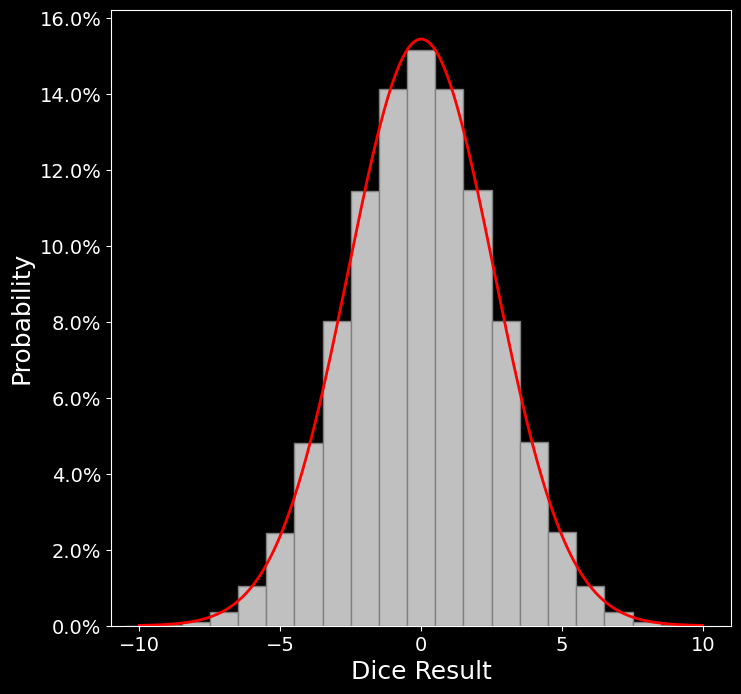
\includegraphics[width=0.95\columnwidth]{10fR}
\end{figure}

\begin{table}[htb]
    \rowcolors{1}{}{lightgray}
    \caption[10fR Probabilities]{10fR Probabilities}
    \label{tab:10fR probabilities}
    \centering
    \begin{tabular}{ccc}
        \toprule
        \textbf{Roll exactly} & \textbf{Chance} & \textbf{one in} \\
        \midrule
        -10/10                & 0.0014\%        & 71000           \\
        -9/9                  & 0.016\%         & 6100            \\
        -8/8                  & 0.088\%         & 1100            \\
        -7/7                  & 0.36\%          & 280             \\
        -6/6                  & 1.0\%           & 96              \\
        -5/5                  & 2.4\%           & 41              \\
        -4/4                  & 4.8\%           & 21              \\
        -3/3                  & 8.0\%           & 13              \\
        -2/2                  & 12\%            & 8.7             \\
        -1/1                  & 14\%            & 7.1             \\
        0                     & 15\%            & 6.6             \\
        \bottomrule
    \end{tabular}
\end{table}

\subparagraph{Probability for rolling a value and lower/higher}


Most of the time it is important to know the probability to at at least a certain
number or higher, or the inverse, the chance to roll a certain number or lower.
Both are important to judge if a \emph{Test} will fail or succeed.

As a rule of thumb, rolling below -5 or above 5 is not happening often. This also
means that \emph{Tests} that only fail when a value smaller than -5 is rolled should
only be done if the success or how well it succeeded or failed is critical for the game.
Instead it can just be assumed that the \emph{Test} succeeded normally.

\begin{figure}[htb]
    \caption{\emph{10fR} Cumulative Probability Distribution}
    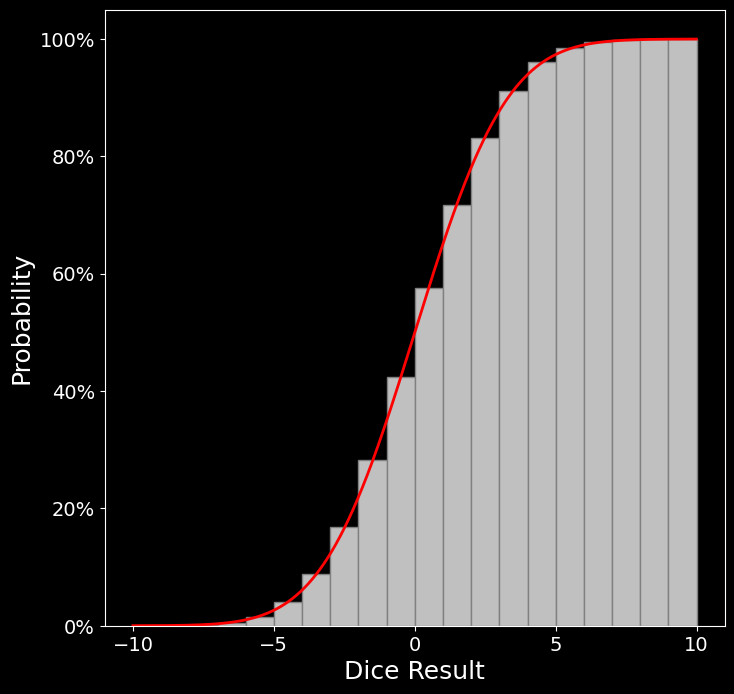
\includegraphics[width=0.95\columnwidth]{10fR_cum}
\end{figure}

\begin{table}[htb]
    \rowcolors{1}{}{lightgray}
    \caption[10fR Cumulative Probabilities]{10fR Cumulative Probabilities}
    \label{tab:10fR cumulative probabilities}
    \centering
    \begin{tabular}{cccc}
        \toprule
        \multicolumn{2}{c}{\textbf{Roll exactly or}} & \multirow{2}{*}{\textbf{Chance}} & \multirow{2}{*}{\textbf{one in}}         \\
        \cmidrule{1-2}
        \textbf{bigger}                              & \textbf{smaller}                 &                                  &       \\
        \midrule
        10                                           & -10                              & 0.0014\%                         & 71000 \\
        9                                            & -9                               & 0.08\%                           & 5600  \\
        8                                            & -8                               & 0.11\%                           & 940   \\
        7                                            & -7                               & 0.46\%                           & 220   \\
        6                                            & -6                               & 1.5\&                            & 66    \\
        5                                            & -5                               & 3.9\%                            & 25    \\
        4                                            & -4                               & 8.8\%                            & 11    \\
        3                                            & -3                               & 17\%                             & 6.0   \\
        2                                            & -2                               & 28\%                             & 3.5   \\
        1                                            & -1                               & 42\%                             & 2.4   \\
        0                                            & 0                                & 58\%                             & 1.7   \\
        \bottomrule
    \end{tabular}
\end{table}

\subsection{Anomalies and Criticals}

The \emph{Result} is not the only quantity that the dice deliver. Another one is
Anomalies and Criticals. They are in principle the same thing, but Criticals are
much more seldom and extreme in their effect.

Criticals and Anomalies are determined only looking at the \emph{5f} roll of either
the player and the game master. This means that both parties in an \emph{Opposed Test}
can generate a Critical or Anomaly at the same time. They happen if multiple dice
show similar symbols.

\paragraph{Anomaly}
\index{Anomaly}
To determine Anomalies the number of similar symbols have to be counted. Every time
4 dice of a \emph{5f} roll show the same symbol, an Anomaly happened.
This can be four ''+'' (Positive Anomaly), four ''-'' (Negative Anomaly) or four
blanks (Neutral Anomaly).

The chance to roll an Anomaly is 4.1\% for any kind of Anomaly. This means that the
chance is 12.3\% to have any kind of Anomaly in a \emph{Test}. The Game Master
needs to decide whether they want to ignore \emph{Anomalies} in an
\emph{Opposing Test}, if the opposing faction is an NPC. The same applies for the other \emph{5f} that are
rolled in a \emph{Unopposed Test}.

\subparagraph{Positive and Negative Anomaly}
\index{Positiv Anomaly}
\index{Negative Anomaly}
The result of a positive or negative Anomaly enhances the outcome of the
\emph{Test} in a positive or negative way respectively, but does not change the
\emph{Result}. The Game Master needs to look at the situation and think of any
positive or negative effects that could happen.

This includes:
\begin{itemize}[parsep=0em]
    \item Taking more/less time of an action in combat that normally can not
          be slowed/sped up
    \item getting into a advantageous/disadvantageous position when performing a
          melee attack
    \item increasing/decreasing connection status of a contact when doing legwork
    \item using less/more resources when crafting an item
\end{itemize}

\subparagraph{Neutral Anomaly}
\index{Neutral Anomaly}
A neutral Moderate Critical should just create unusual side effects to an outcome.
Again the Game Master should be free to invent anything coming to their mind.

For example:
\begin{itemize}[parsep=0em]
    \item A
    \item b
    \item c
\end{itemize}

\paragraph{Critical}
\index{Critical}
Criticals happens if all 5 dice of a \emph{5f} show the same symbol. As with Anomalies
there are positive, negative and neutral Criticals. Both the chance and the effect of
a Critical are much more radical than an Anomaly.

The chance to roll any kind of Critical is 0.4\%.

\subparagraph{Positive Critical}
\index{Positive Critical}

If there is a remote chance of the \emph{Test} succeeding, it will. This does not
allow \emph{PC} to do things that are impossible like surviving an atomic blast or
succeeding in a wrestling match with a dragon, but anything close to that.

\subparagraph{Negative Critical}
\index{Negative Critical}

The \emph{Test} fails and it fails spectacularly. The Game Master is free to invent
any convenient explanations. There is always a way something can fail.

\subparagraph{Neutral Critical}
\index{Neutral Critical}

The \emph{Result} of the \emph{Test} is not affected, but something very strange
happens. The Game Master can do whatever they see fit.


\subsection{Non Blanks}

The Non Blanks of \emph{5f}is calculated by counting all the ''+'' and ''-''
symbols, resulting in a number from 0 to 5.

If the Non Blanks need to be calculated from a \emph{Test} this is denoted as:
\[ \textit{5fN} \]
\index{5fN}
Note that does not mean that an additional \emph{5f}need to be rolled in addition to
the \emph{10f} of the \emph{Test} itself, but instead use the \emph{5f}from the
existing \emph{10f}roll.

The Non Blanks are used for various secondary purposes of a dice roll.

\begin{figure}[htb]
    \caption{\emph{5fN} Probability Distribution}
    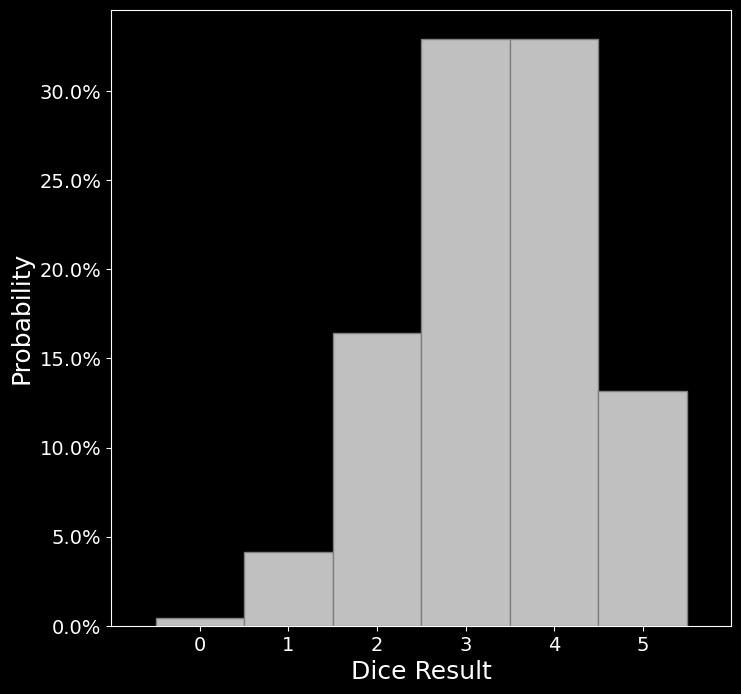
\includegraphics[width=0.95\columnwidth]{5fN}
\end{figure}

\begin{table}[htb]
    \rowcolors{1}{}{lightgray}
    \caption[5dN Probabilities]{5dN Probabilities}
    \label{tab:5dN probabilities}
    \centering
    \begin{tabular}{ccc}
        \toprule
        \textbf{Roll exactly} & \textbf{Chance} & \textbf{one in} \\
        \midrule
        5                     & 13\%            & 7.6             \\
        4                     & 33\%            & 3.0             \\
        3                     & 33\%            & 3.0             \\
        2                     & 16\%            & 6.1             \\
        1                     & 4.1\%           & 24              \\
        0                     & 0.4\%           & 240             \\
        \bottomrule
    \end{tabular}
\end{table}

\section{Tests}
\index{Test}

A test determines the outcome of a certain action, which has a certain probability to
fail and which has an important impact on the game session if it fails. Tests should
not be rolled if it is clear that the test will succeed, like in the case of opening
a door. Tests should also not be rolled if the result is irrelevant for the game
session, like when a character is trying to beat a popular game in their spare time.

Every time the outcome of an action is, given the capabilities of the acting
character, in doubt, or if the result needs to be quantified, a \emph{Test} is rolled.

\subsection{Test Anatomy}

All Tests in Pink Trenchcoat look like the following:

\begin{equation}
    \begin{split}
        \textit{Test Quality} = {} & \textit{10fR}  + \textit{Ability Score(s)} \\
        & + \textit{Modifiers(s)}
    \end{split}
\end{equation}


The \emph{10fR} was already explained in the previous section.

\paragraph{Ability Score}
\index{Ability Score}

The Ability Score is a number giving the proficiency of the person or entity that
performs the \emph{Test} to achieve the result. The higher, the better.

Normally Ability Scores are either \emph{Attributes} or \emph{Skills} of a character.

\subparagraph{Limits}
\index{Limit}

Sometimes tools and other situational effects are not modeled as a \emph{Modifier}
that is added or subtracted but as a \emph{Limit} to the \emph{Ability Score}. In
case the \emph{Ability Score} can not be higher than the \emph{Limit}.

\emph{Limits} to the \emph{Ability Score} are noted as follows:

\begin{equation}
    \textit{Ability Score}(\textit{Limit})
\end{equation}

\paragraph{Modifier}

\emph{Modifier} can be anything from a threshold that needs to be achieved to
circumstantial \emph{Modifiers} like visual conditions, tools or wounds that can
change the result of a \emph{Test}. If a \emph{Modifier} is helping the
\emph{Character} performing the \emph{Test}, like good tools, or support from friends,
it is positive. If it is an obstacle of problem for the \emph{Character} performing
the \emph{Test}, the \emph{Modifier} is negative.

\paragraph{Test Quality}
\index{Test Quality}
\index{TQ}

The \emph{Test Quality} ot \emph{TQ} is the value that results from adding the
\emph{10fR} the \emph{Ability Score} and the \emph{Modifiers}. If the
\emph{Test Quality} is zero or positive, the \emph{Test} succeed, if it negative
it failed. The higher the \emph{Test Quality} the better the result and the lower
the \emph{Test Quality} the worse the failure.


\begin{table}[htb]
    \rowcolors{1}{}{lightgray}
    \caption[Test Quality]{Test Quality}
    \label{tab:test quality}
    \centering
    \begin{tabular}{cl}
        \toprule
        \textbf{TQ} & \textbf{Description} \\
        \midrule
        < -9        & Epic Fail            \\
        -7 to -9    & Severe Failure       \\
        -4 to -6    & Decisive Failure     \\
        -1 to -3    & Failure              \\
        0           & Barely made it       \\
        1 to 3      & Acceptable           \\
        4 to 6      & Good Result          \\
        7 to 9      & Exceptional          \\
        > 9         & Epic Success         \\
        \bottomrule
    \end{tabular}
\end{table}

\subsection{Unopposed Tests}
\index{Unopposed Test}

In an \emph{Unopposed Tests} a \emph{Character} is not testing against another
\emph{Character} but against the environment. Typical \emph{Unopposed Tests} include:

\begin{itemize}[parsep=0em]
    \item crafting something
    \item climbing a wall
    \item running fast
    \item remembering something
\end{itemize}

In this case, the \emph{Ability Score} is just the relevant value from the
\emph{Character} and the \emph{Modifier} is the difficulty of the task plus any
additional situational \emph{Modifiers}.

This rule system defines the \emph{Ability Scores} to use in an
\emph{Unopposed Test} in the following notation:

\begin{equation}
    \textit{Ability Score}_\textit{Acting Character} \; + \textit{Modifier}
\end{equation}

In case of a climbing test for a given wall, that would be:

\begin{equation*}
    \textit{Climbing} \; -6
\end{equation*}

\subsection{Opposed Tests}
\index{Opposed Test}

If two \emph{Characters} are fighting against each other, either literally in melee
combat or figuratively when one \emph{Character} tries to sneak by and the other to
spot the sneaker, an \emph{Opposed Test} is called for. In this case, both involved
\emph{Characters} \emph{Ability Scores} are used. The definition of the \emph{Test}
explains which values of a \emph{Character} are used, as this can be the same, in the
case of melee combat or be different in the case of sneaking.

This rule system defines the \emph{Ability Scores} to use in an
\emph{Opposed Test} in the following notation:

\begin{equation}
    \textit{Ability Score}_\textit{Attacker} \; \textit{vs.} \; \textit{Ability Score}_\textit{Defender}
\end{equation}

In case of melee combat this would mean:

\begin{equation*}
    \textit{Melee Combat} \; \textit{vs.} \; \textit{Melee Combat}
\end{equation*}

In case of sneaking it would mean:

\begin{equation*}
    \textit{Stealth} \; \textit{vs.} \; \textit{Perception}
\end{equation*}

The final \emph{Test Quality} is then calculated as follows:

\begin{equation}
    \begin{split}
        \textit{Test Quality} = {} & \textit{10fR} \\
        & + \textit{Ability Score}_\textit{Attacker} \\
        & + \textit{Modifiers(s)}_\textit{Attacker} \\
        & - \textit{Ability Score}_\textit{Defender} \\
        & - \textit{Modifiers(s)}_\textit{Defender} \\
    \end{split}
\end{equation}


Ties\index{Ties} are broken either by bespoke tie breakers given in the specific rules section,
or, and if those tie breakers still end in a tie, by the\emph{Game Master}. They
can decide to either flip a coin or decide for themselves.

\subsection{Supported Tests}\index{Supported Test}

If one or more \emph{Characters} are helping another \emph{Character} to do a task
that can not be split into subtasks, but all characters have to do the full task,
this is a \emph{Supported Test}.

\begin{itemize}[parsep=0em]
    \item climbing a wall together
    \item helping a character to sneak
    \item crossing a mine-field
\end{itemize}

In this case the \emph{Ability Score} for the \emph{Supported Test} is the average
\emph{Ability Score} of all the \emph{Characters} involved. The \emph{Modifiers}
for the \emph{Supported Test} are the average
\emph{Modifiers} of all the \emph{Characters} involved -1.

The \emph{Game Master} decides which \emph{Tests} can be supported.

\subsection{Collaborative Tests}
\index{Collaborative Test}

If one or more \emph{Characters} are working together, distributing the work to
perform a task that can be broken down into independent parts this is a
\emph{Team-Play Test}. The goal is to either increase the quality of the result, or
to speed up the process by using less \emph{Task Time}.

\begin{itemize}[parsep=0em]
    \item crafting an item
    \item collecting information
    \item repairing a vehicle
    \item summoning a spirit
\end{itemize}

In this case the \emph{Ability Score} for the \emph{CollaborativeTest} is the average
\emph{Ability Score} of all the \emph{Characters} involved. The \emph{Modifiers}
for the \emph{Collaborative Test} are the average
\emph{Modifiers} of all the \emph{Characters} with an additional benefit depending
on the number of \emph{Characters} working in the \emph{Test}.

\begin{table}[htb]
    \rowcolors{1}{}{lightgray}
    \caption[CollaborativeTest]{Collaborative Test}
    \label{tab:team-play test}
    \centering
    \begin{tabular}{cc}
        \toprule
        \textbf{Characters} & \textbf{Modifier} \\
        \midrule
        3                   & +1                \\
        10                  & +2                \\
        100                 & +3                \\
        1000                & +4                \\
        \bottomrule
    \end{tabular}
\end{table}

The \emph{Game Master} decides which \emph{Tests} can be \emph{Collaborative Tests}.

\subsection{Task Time}
\index{Task Time}

In most \emph{Tests} a \emph{Character} can spend more ore less \emph{Task Time} to
do the task better or achieve an outcome faster. In the case of spending more
\emph{Task Time}, this will either make a success possible or allow for a better
result.

\begin{table}[htb]
    \rowcolors{1}{}{lightgray}
    \caption[Extra Time]{Extra Time}
    \label{tab:extra time}
    \centering
    \begin{tabular}{cc}
        \toprule
        \textbf{Time Multiplier} & \textbf{Modifier} \\
        \midrule
        x0.5                     & -6                \\
        x0.7                     & -3                \\
        x3                       & +1                \\
        x10                      & +2                \\
        x100                     & +3                \\
        x1000                    & +4                \\
        \bottomrule
    \end{tabular}
\end{table}

If not explicitly allowed or disallowed by the rules the \emph{Game Master}
decides whether spending more or less \emph{Task Time} is possible.

\section{Thoughts and Philosophy}

The main idea behind the use of 10f is are th follows:

\begin{itemize}[parsep=0em]
    \item easy calculable expectation value
    \item possibility of suspense
    \item possibly only one roll per decision
\end{itemize}


\paragraph{Expectations}
It should be easy to calculate the average and preferably also the most common
outcome of a \emph{Test}. In this rule-system both are the same and are extremely
easy to judge, being zero. The average outcome of a \emph{Test} is thus always
the sum of \emph{Ability Score} and \emph{Modifiers}.

It is also important that the average outcome is occurring more often than the
extremes. This is not the case in linear systems like d20 where the extremes of
1 and the 20 are just as probable as the average 10 or 11.
This is important because although a lot of tings are handled by rules,
the vast majority of expectations about a game come from the real world,
which mostly follows gaussian-like distributions and thus shape player expectations.

\paragraph{Suspense}

\paragraph{One Roll}
This is not only design concept, but should also be the philosophy of each
\emph{Game Master}. If there is no decision between two \emph{Tests}, the second
test is unnecessary and should be avoided.
A big \emph{Test} should only be divided into smaller more granular \emph{Tests}
it is both
interesting for the \emph{Players} and there are decisions between the \emph{Tests}.
Otherwise just one general Test should be made.